% Exercise Template
% A LaTeX template for typesetting exercise in Persian (with cover page).
% By: Reza Adinepour
% Github: github.com/rezaAdinepour

\documentclass[12pt]{exam}

\usepackage{setspace}
\usepackage{listings}
\usepackage{graphicx,wrapfig}
\usepackage{caption}
\usepackage{subcaption}
\usepackage{multirow}
\usepackage{matlab-prettifier}
\usepackage{amsmath}
\usepackage{multicol}
\usepackage[hidelinks]{hyperref}



\usepackage[utf8]{inputenc}
\usepackage{fourier} 
\usepackage{array}
\usepackage{makecell}

\renewcommand\theadalign{bc}
\renewcommand\theadfont{\normalsize}
\renewcommand\theadgape{\Gape[4pt]}
\renewcommand\cellgape{\Gape[4pt]}


\usepackage[margin=25mm]{geometry}
\usepackage{xepersian}
\settextfont{XB Niloofar}

\newcommand{\class}{\ThesisClass}

\singlespacing
\parindent 0ex

\begin{document}


% -------------------------------------------------------
%  Thesis Information
% -------------------------------------------------------

\newcommand{\ThesisType}
{سمینار}  % پایان‌نامه / رساله
\newcommand{\ThesisDegree}
{کارشناسی ارشد گرایش معماری کامپیوتر}  % کارشناسی / کارشناسی ارشد / دکتری
\newcommand{\ThesisMajor}
{مهندسی کامپیوتر}  % مهندسی کامپیوتر
\newcommand{\ThesisTitle}
{تمرین شبیه‌سازی اول}
\newcommand{\ThesisAuthor}
{نام دانشجو\\شماره دانشجویی}
\newcommand{\ThesisClass}
{درس فناوری های حافظه\\دکتر حامد فربه}
\newcommand{\ThesisSemester}
{CE5431 | بهار ۱۴۰۳}
\newcommand{\ThesisDate}
{اسفند 1402}
\newcommand{\ThesisDepartment}
{دانشکده مهندسی کامپیوتر}


\newcommand{\ThesisGroupNameI}
{مرتضی عادلخانی (\href{mailti:madelkhani@aut.ac.ir}{\textcolor{blue}{madelkhani@aut.ac.ir}})}
\newcommand{\ThesisGroupNameII}
{سارا زمانی (\href{mailti:sara.zamani73@aut.ac.ir}{\textcolor{blue}{sara.zamani73@aut.ac.ir}})}


\newcommand{\ThesisUniversity}
{دانشگاه صنعتی امیرکبیر}

% -------------------------------------------------------
%  English Information
% -------------------------------------------------------

\newcommand{\EnglishThesisTitle}{A Standard Template for Course Exercise}


\pagestyle{empty}

\begin{center}

\includegraphics[scale=0.18]{images/aut-fa2.png}

%\vspace{0.5cm}
%\ThesisUniversity \\[-0.3em]
%\vspace{0.5cm}
\large\ThesisDepartment

\begin{large}
\vspace{0.5cm}


%\ThesisMajor

\end{large}

\vspace{1cm}


{\large\textbf{\ThesisClass}}
\vspace{1cm}

%{نگارش}\\[.5em]
{\large\textbf{\ThesisAuthor}}


\vspace{1.5cm}

{\LARGE\textbf{\ThesisTitle}}\\ 
\vspace{2cm}





% \begin{latin}
% {\Large\textbf\EnglishThesisTitle}
% \end{latin}

{تدریسیار:}\\[.8em]

\ThesisGroupNameI \\
\ThesisGroupNameII



\vspace{3cm}



\ThesisSemester

\end{center}

\newpage


% These commands set up the running header on the top of the exam pages
\pagestyle{head}
\firstpageheader{}{}{}
\runningheader{صفحه \thepage\ از \numpages}{}{\class}
\runningheadrule

\vspace{0pt}


\begin{questions}
	\pointpoints{نمره}{نمره}
	
	
	\question 
	نام چهار شبیه‌ساز که در زمینه فناوری های حافظه مورد استفاده قرار می‌گیرند را نام ببرید و آنها را بررسی کنید. زبان برنامه نویسی هرکدام، برنامه هایی که می‌تواند پشتیبانی کند و چالش های احتمالی را بیان کنید. همچنین مزایا و معایب هرکدام را بررسی کنید


شبیه ساز‌هایی که در این تمرین بررسی شده است:



\begin{center}
	\begin{tabular}{||c c c c c c||} 
		\hline
		نام شبیه‌ساز & کاربرد & زبان برنامه نویسی & مزایا & معایب & سایت \\ [0.5ex] 
		\hline\hline
		CACTI & \thead{تحلیل و شبیه سازی \\حافظه‌های \\ نهان\footnote{Cache} بزرگ} & C/C++ & سرعت بالا & \thead{فاصله زیاد نسبت \\به دنیای واقعی} & \href{https://www.hpl.hp.com/research/cacti/}{\textcolor{magenta}{Website}} \\ 
		\hline
		NVSIM & \thead{طراحی و شبیه‌سازی \\ حافظه های غیر فرار} & C/C++ & \thead{پشتیبانی از \\ حافظه های جدید} & \thead{عدم وجود نسخه \\ رسمی از شبیه‌ساز} & \href{http://nvsim.org/}{\textcolor{magenta}{Website}} \\
		\hline
		DRAMSim & \thead{مدلسازی حافظه\\ های پویا\footnote{Dynamic}} & C/C++ & \thead{پشتیبانی از \\ تکنولوژی های جدید} & \thead{عدم ارائه \\ گزارش جامع} & \href{https://par.nsf.gov/servlets/purl/10216399}{\textcolor{magenta}{Website}} \\
		\hline
		SimpleScaler & \thead{شبیه‌سازی اجزای\\کامپیوتر} & C & \thead{شبیه‌سازی کامل\\یک سیستم کامپیوتری} & \thead{عدم ارائه\\تحلیل های کامل} & \href{www.simplescalar.com}{\textcolor{magenta}{Website}} \\
		[1ex] 
		\hline
	\end{tabular}
\end{center}





%\begin{center}
%	\begin{tabular}{||c c c c c c||} 
%		\hline
%		نام شبیه‌ساز & کاربرد & زبان برنامه نویسی & مزایا & معایب & سایت \\ [0.5ex] 
%		\hline\hline
%		CACTI & \thead{تحلیل و شبیه سازی \\حافظه‌های \\ نهان\footnote{Cache} بزرگ} & C/C++ & سرعت بالا & \thead{فاصله زیاد نسبت \\به دنیای واقعی} & \href{https://www.hpl.hp.com/research/cacti/}{\textcolor{magenta}{Website}} \\ 
%		\hline
%		NVSIM & \thead{طراحی و شبیه‌سازی \\ حافظه های غیر فرار} & C/C++ & \thead{پشتیبانی از \\ حافظه های جدید} & \thead{عدم وجود نسخه \\ رسمی از شبیه‌ساز} & \href{http://nvsim.org/}{\textcolor{magenta}{Website}} \\
%		\hline
%		DRAMSim & \thead{مدلسازی حافظه\\ های پویا\footnote{Dynamic}} & C/C++ & \thead{پشتیبانی از \\ تکنولوژی های جدید} & \thead{عدم ارائه \\ گزارش جامع} & \href{https://par.nsf.gov/servlets/purl/10216399}{\textcolor{magenta}{Website}} \\
%		\hline
%		SimpleScaler & \thead{شبیه‌سازی اجزای\\کامپیوتر} & C & \thead{شبیه‌سازی کامل\\یک سیستم کامپیوتری} & \thead{عدم ارائه\\تحلیل های کامل} & \href{www.simplescalar.com}{\textcolor{magenta}{Website}} \\
%		\hline
%		
%		DiskSim & & & & & \href{https://www.pdl.cmu.edu/DiskSim/index.shtml}{\textcolor{magenta}{Website}} \\ 
%		\hline
%		Ramulator & & & & & \href{https://arxiv.org/abs/2308.11030}{\textcolor{magenta}{Website}} \\
%		\hline
%		
%		OpenRAM & & & & & \href{https://openram.org/}{\textcolor{magenta}{Website}} \\
%		\hline
%		HSPICE & & & & & \href{https://www.synopsys.com/}{\textcolor{magenta}{Website}} \\
%		\hline
%		Gem5 & & & & & \href{https://www.gem5.org/}{\textcolor{magenta}{Website}} \\ [1ex] 
%		\hline
%	\end{tabular}
%\end{center}




\section{شبیه‌ساز CACTI}
اولین بار این شبیه‌ساز در سال ۱۹۹۳ توسط دکتر جوپی\footnote{Jouppi Dr.} و دکتر ویلتون\footnote{Wilton Dr.} در یکی از آزمایشگاه های شرکت HP توسعه داده شد. CACTI ابزاری تحلیلی\footnote{Analytical} است. به طور کلی عملکرد این شبیه ساز را می‌توان به دو دسته زیر تقسیم کرد:

\begin{enumerate}
	\item شبیه‌سازی و مدلسازی دسترسی به حافظه
	\item مدلسازی انواع مسیر‌ها و سیم ها
\end{enumerate}



\begin{figure}
	\centering
	\begin{subfigure}[b]{0.3\textwidth}
		\centering
		\includegraphics[width=\textwidth]{images/img1}
		\caption{ساختار منطقی Cache}
		\label{ساختار منطقی Cache}
	\end{subfigure}
	\hfill
	\begin{subfigure}[b]{0.3\textwidth}
		\centering
		\includegraphics[width=\textwidth]{images/img2}
		\caption{ساختار فیزیکی Cache}
		\label{ساختار فیزیکی Cache}
	\end{subfigure}
	\hfill

	\caption{ساختار منطقی و فیزیکی Cache}
	\label{ساختار منطقی و فیزیکی Cache}
\end{figure}






 اگر چه این شبیه‌ساز همه سلسله مراتب حافظه را شبیه‌سازی می‌کند اما همانطور که از دو حرف اول اسم این شبیه‌ساز مشخص است\footnote{Architecture Cache}، کاربرد اصلی این شبیه‌ساز در تحلیل حافظه‌های نهان است.
 
 این شبیه‌ساز می‌توان سطوح مختلف حافظه نهان، سیسات های مختلف انجمنی\footnote{Associativity} و سیاست های جایگزینی\footnote{policies Replacement} و ... را برای ایجاد تغییرات و شبیه سازی فراهم کند.

در بخش اول، مجموعه ای از پارامتر‌های حافظه «به خصوص حافظه نهان\footnote{Cache}» را به عنوان ورودی می‌گیرد و پارامتر‌هایی مثل زمان دسترسی\footnote{time Access}، توان\footnote{Power}، زمان چرخه\footnote{time Sycle}، مساحت\footnote{Area} و ... را محاسبه می‌کند.

در بخش دوم، CACTI قابلیت تست و مدل‌سازی تاخیر، توان، مساحت و ... در مسیر‌های حافظه، مانند خط آدرس\footnote{line Word} و خطوط داده\footnote{line Bit} را دارد.\\


 
CACTI به دو صورت در دسترس است:
\begin{enumerate}
	\item \footnote{\href{https://quid.hpl.hp.com:9081/cacti/}{\textcolor{magenta}{\lr{quid.hpl.hp.com:9081/cacti/}}}}وب
	\item سورس کد C++ 
\end{enumerate}

که در ادامه نحوه نصب و کار با شبیه ساز 0.7 CACTI «آخرین ورژن» را توضیح خواهیم داد. برای دانلود و نصب شبیه‌ساز CACTI بر می‌توان طبق مراحل زیر عمل کرد:

\subsection{دانلود و نصب}


در گام اول می‌بایست وابستگی\footnote{Dependency} های مورد نیاز را نصب کرد. برای نصب به صورت زیر عمل می‌کنیم:\\
\begin{latin}
	\texttt{\textcolor{blue}{\$} sudo apt-get update}\\
	\texttt{\textcolor{blue}{\$} sudo apt-get install build-essential}
\end{latin}



\subsubsection{دانلود شبیه‌ساز}
پس از نصب Dependency ها باید سورس کد شبیه‌ساز را دانلود کنیم. به صورت زیر عمل می‌کنیم:\\

\begin{latin}
	\texttt{\textcolor{blue}{\$} git clone https://github.com/HewlettPackard/cacti.git}
\end{latin}



\subsubsection{بیلد شبیه‌ساز}
پس از Clone کردن مخزن\footnote{Repository}، به دایرکتوری مخزن میرویم و شبیه‌ساز را Build می‌کنیم: \\

\begin{latin}
	\texttt{\textcolor{blue}{\$} cd CACTI}\\
	\texttt{\textcolor{blue}{\$} make}
\end{latin}

اگر شبیه‌ساز به درستی Build شود، خروجی ترمینال به صورت زیر خواهد شد:

\begin{figure}[h]
	\centering
	\includegraphics[width=1\textwidth]{images/img3}
	\caption{Build موفقیت آمیز}
	\label{بیلد موفق ککتای}
\end{figure}


\subsubsection{تنظیم پارامتر‌های Cache}
در ورژن های قدیمی تر CACTI می‌توانستیم پارامتر‌های Cache را به صورت Command درون ترمینال تنظیم کنیم. اما از ورژن ۶ به بعد نرم افزار تمامی کانفیگ ها به درون فایلی با نام \texttt{cache.cfg} منتقل شده است. «شکل \textcolor{blue}{\ref{حتوای درون فایل کش}}»

\begin{figure}[h]
	\centering
	\includegraphics[width=1\textwidth]{images/img4}
	\caption{محتوای درون فایل \texttt{cache.cfg}}
	\label{حتوای درون فایل کش}
\end{figure}

پارامتر‌های مختلفی مانند سایز کش، size Block ، نوع تکنولوژی و ... وجود دارد که ما تغییری در آن ایجاد نمی‌کنیم تنظیمات پیش‌فرض\footnote{Default} را می‌پذیریم. \newpage



\subsubsection{اجرای شبیه‌سازی}
پس از ذخیره تنظیمات با دستور زیر، شبیه‌سازی را اجرا می‌کنیم:\\

\begin{latin}
	\texttt{\textcolor{blue}{\$} ./cacti -infile cache.cfg}\\
\end{latin}

شبیه سازی با موفقیت انجام می‌شود و خروجی های تحلیل را به صورت «شکل \textcolor{blue}{\ref{خروجی شبیه‌سازی ککتای}}» گزارش می‌دهد.

درون این مخزن، تنظیمات دیگری همچون:
\begin{enumerate}
	\item تنظیمات DRAM
	\item تنظیمات حافظه DDR3
	\item و ...
\end{enumerate}

نیز وجود دارد که می‌توان آن‌ها را نیز همانند دستور قبل شبیه‌سازی کرد.

\begin{figure}[h]
	\centering
	\includegraphics[width=1\textwidth]{images/img5}
	\caption{خروجی شبیه‌سازی}
	\label{خروجی شبیه‌سازی ککتای}
\end{figure}


\subsection{\textcolor{green}{مزایا}}

\begin{enumerate}
	\item \textbf{عام منظوره بودن:}\\
	شبیه‌ساز CACTI تمام اجزای یک حافظه را تحلیل و شبیه‌سازی می‌کند و صرفا مختص به حافظه‌های نهان نیست. همچنین تخمینی از توان مصرفی مدار نیز ارائه می‌دهد که طراح می‌تواند با توجه به آن طراحی خود را از نظر توان مصرفی بهینه‌سازی کند.
	
	\item \textbf{سرعت بالا: }\\
	این شبیه‌ساز محاسبات تخمینی مناسبی از مصرف انرژی حافظه، مساحت مصرفی و تاخیر ها برای پیکر‌بندی های\footnote{Configurations} های مختلف ارائه می‌کند که همین محاسبات تخمینی باعث افزایش سرعت در انجام شبیه‌سازی می‌شود و دید مناسبی به طراح برای ادامه روند طراحی می‌دهد.
	
	\item \textbf{انعطاف پذیری بالا در شخصی سازی: }\\
	طراح می‌تواند بسته به نیاز و طراحی خود، به تمام قسمت های حافظه دسترسی داشته باشد و آنها را متناسب با نیاز خود تغییر دهد.
\end{enumerate}


\subsection{\textcolor{red}{معایب}}
\begin{enumerate}
	\item \textbf{عدم انجام محاسبات دقیق: }\\
	شبیه‌ساز CACTI برای افزایش سرعت شبیه‌سازی و جلوگیری از پیچیده شدن مدل ارائه شده به آن، یک سری ساده سازی ها انجام می‌دهد که همین امر باعث شده است که این ابزار صرفا در محیط اکادمیک مورد استفاده قرار گیرد و استفاده آنچنانی ای در صنعت نداشته باشد.
	
	\item \textbf{موازی نبودن روند دنیای حافظه‌ها و امکانات شبیه‌ساز}\\
عدم توانایی و تحلیل حافظه‌های نو ظهور مانند DDR5 و RERAM و CAM


	\item \textbf{بلادرنگ\footnote{Real-Time} نبودن: }\\
	اگر در زمان کار یک حافظه بخواهیم تغییراتی در آن انجام دهیم و همانجا تغییرات ناشی از آن را مشاهده کنیم. این امر با شبیه‌ساز CACTI امکان پذیر نمی‌باشد.
	
	\item \textbf{عدم وجود Community گسترده و قوی: }\\
	متاسفانه برای آموزش و تحلیل این شبیه‌ساز برای مبتدیان منابع و Community بسیار محدودی وجود دارد که می‌تواند باعث سردرگمی شود.
\end{enumerate}












\section{شبیه‌ساز NVSIM}
شبیه ساز NVSIM ابزاری برای تحلیل و شبیه‌سازی حافظه‌های غیرفرار\footnote{Non-volatile} است که عمدتا برای تحلیل و تخمین مساحت، توان و انرژی مصرفی در حافظه های غیر فرار استفاده می‌شود.

برخلاف شبیه‌ساز CACTI ، شبیه‌ساز NVSIM از شبیه‌سازی و تحلیل حافظه‌های نو ظهور هم پشتیبانی می‌کند. حافظه هایی که در NVSIM قابلیت تحلیل دارند را می‌توان به صورت زیر دسته‌بندی کرد:

\begin{latin}
	\begin{enumerate}
		\item NAND Flash
		\item SRAM
		\item DRAM
		\item PCM (Phase Change Memory)
		\item STT RAM (Spin Torque Transfer RAM)	
		\item ReRAM (Resistive RAM)
		\item FBDRAM (Floating Body Dynamic RAM)
		\item eDRAM	
	\end{enumerate} 
\end{latin}

شبیه‌ساز NVSIM از اصول طراحی مشابه با CACTI استفاده می‌کند اما بر خلاف CACTI انعطاف پذیری بیشتری در سازماندهی بانک های حافظه دارد. چنین انعطاف پذیری ای برای حافظه‌های غیر فرار نوظهور ضروری است چرا که وضعیت اکثر حافظه های نوظهور نا شناخته است و این انعطاف پذیری دست طراح را برای بررسی بیشتر بخش های مختلف حافظه باز می‌کند.

همانند CACTI این شبیه‌ساز نیز با زبان C++ نوشته شده است و فایل کانفیگ حافظه را در دو فرمت \texttt{.cfg} و \texttt{.cell} دریافت می‌کند.

شبیه‌ساز NVSIM از داده های ITRS برای مدل های خود استفاده می‌کند. این ابزار فناوری های 180nm ، 120nm ، 90nm ،  65nm ، 45nm و 32nm را پوشش می‌دهد و از ترانزیستور کارایی‌بالا\footnote{performance High} ، توان عملیاتی کم\footnote{operation power Low} و power stand-by Low استفاده می‌کند.

«شکل \textcolor{blue}{\ref{سازماندهی سطوح حافظه در NVSIM}}» سازماندهی سطوح حافظه را در NVSIM نشان می‌دهد.

\begin{figure}[h]
	\centering
	\includegraphics[width=1\textwidth]{images/img10}
	\caption{سازماندهی سطوح حافظه در NVSIM}
	\label{سازماندهی سطوح حافظه در NVSIM}
\end{figure}

همانطور که مشخص است،‌ سلسله مراتب حافظه در NVSIM از سه سطح بانک\footnote{Bank} ، مت\footnote{Mat} و زیرآرایه\footnote{array Sub} تشکیل می‌شود.

بانک ساختار سطح بالاییست که در NVSIM مدل شده است. یک تراشه حافظه غیر فرار می‌تواند چندین بانک داشته باشد. بانک یک واحد حافظه کاملا مهم و کاربردی است و می‌توان آن را به طور مستقل اداره کرد. در هر بانک سلول ها در ساختار H-tree و یا با گذرگاه\footnote{bus} هایی به هم متصل شده اند.

هر مت از چندین زیر آرایه و یک بلوک پیش‌رمزگشا\footnote{decoder Pre} تشکیل می‌شود.\\

شبیه‌ساز NVSIM سه نوع طراحی حافظه را مدل‌سازی می‌کند:
\begin{latin}
	\begin{enumerate}
		\item RAM
		\item Set assiocative cache
		\item CAM
	\end{enumerate}
\end{latin}








برای دانلود و نصب این شبیه‌ساز می‌توان به صورت زیر عمل کرد:

\subsection{دانلود و نصب}

ابتدا می‌بایست مخزن NVSIM را دریافت کنیم. این کار را می‌توان به صورت زیر انجام داد: \\

\begin{latin}
	\texttt{\textcolor{blue}{\$} git clone https://github.com/lpentecost/nvsim-merged} \\
\end{latin}

پس از دریافت کامل NVSIM با دستور زیر وارد فایل مخزن می‌شویم: \\

\begin{latin}
	\texttt{\textcolor{blue}{\$} cd nvsim-merged} \\
\end{latin}

حال می‌بایست شبیه ساز را بیلد کنیم: \\

\begin{latin}
	\texttt{\textcolor{blue}{\$} make} \\
\end{latin}

اگر شبیه‌ساز به درستی بیلد شود، خروجی می‌بایست به صورت زیر شود:

\begin{figure}[h]
	\centering
	\includegraphics[width=1\textwidth]{images/img6}
	\caption{بیلد موفق NVSIM}
	\label{بیلد موفق NVSIM}
\end{figure}


\subsection{تنظیمات فایل کانفیگ}

همانند CACTI می‌بایست فایل کانفیگ را به شبیه‌ساز بدهیم. برای انجام این کار از فایل کانفیگ \texttt{sample.cfg} که به صورت پیش‌فرض وجود دارد استفاده می‌کنیم. این فایل، فایل کانفیگ یک Memristor ۶۴ بیتی‌ست.

محتویات درون فایل \texttt{sample.cfg} به صورت زیر است: «شکل \textcolor{blue}{\ref{فایل کانفیگ سمپل}}»

\begin{figure}[h]
	\centering
	\includegraphics[width=1\textwidth]{images/img7}
	\caption{فایل کانفیگ \texttt{sample.cfg}}
	\label{فایل کانفیگ سمپل}
\end{figure}


\subsection{اجرای شبیه‌سازی}
پس از تنظیمات کانفیگ با دستور زیر می‌توان شبیه‌سازی را انجام داد:
\begin{latin}
	\texttt{\textcolor{blue}{\$} ./nvsim sample.cfg} \\
\end{latin}

به جای \texttt{sample.cfg} می‌توان هر فایل کانفیگ دیگری را قرار داد. دقایقی طول خواد کشید تا شبیه‌سازی به اتمام برسد. پس از تمام شدن شبیه‌سازی خروجی آن به صورت زیر خواهد بود: «شکل \textcolor{blue}{\ref{خروجی شبیه‌سازی NVSIM}}»

\begin{figure}[h]
	\centering
	\includegraphics[width=1\textwidth]{images/img8}
	\caption{خروجی شبیه‌سازی}
	\label{خروجی شبیه‌سازی NVSIM}
\end{figure}

همانطور که از «شکل \textcolor{blue}{\ref{خروجی شبیه‌سازی NVSIM}}» نشخص است، خروجی شبیه سازی شامل تحلیلی از مساحت\footnote{Area} ، زمان‌بندی\footnote{Timing} و توان مصرفی حافظه است.




\subsection{\textcolor{green}{مزایا}}
\begin{enumerate}
	\item \textbf{امکان شبیه‌سازی حافظه های جدید: }\\
	شبیه‌ساز NVSIM قادر به شبیه‌سازی و تحلیل حافظه‌های جدید و نو ظهوری مثل ReRAM ، STTRAM و ... می‌باشد.
	
	
	\item \textbf{قابلیت تغییر و شخصی سازی در سطوح پایین: }\\
	شبیه‌ساز NVSIM با طراح این امکان و دسترسی را می‌دهد تا تغییرات خود را در سطح بانک ها و سلول های حافظه اعمال کند.
	
	\item \textbf{متن باز بود: }\\
	شبیه‌ساز NVSIM متن باز است و هرکس می‌تواند آن را متناسب با نیاز های خود توسعه دهد.
\end{enumerate}


\subsection{\textcolor{red}{معایب}}
\begin{enumerate}
	\item \textbf{بلادرنگ نبودن: }\\
	اگر در زمان کار یک حافظه بخواهیم تغییراتی در آن انجام دهیم و همانجا تغییرات ناشی از آن را مشاهده کنیم. این امر با شبیه‌ساز NVSIM امکان پذیر نمی‌باشد.
	
	\item \textbf{عدم وجود نسخه رسمی: }\\
	تمام نسخه های موجود در اینترنت نسخه های Modify شده هستند. و یک نسخه اصلی از شرکت سازنده موجود نیست.
\end{enumerate}





\section{شبیه‌ساز DRAMSIM}
مدلسازی و شبیه‌سازی دقیق حافظه های پویا\footnote{Dynamic} از این جهت مهم است که تکنولوژی سعی بر آن دارد که CPU و DRAM را به صورت مجتمع در یک تراشه ارائه دهد. این کار تراکم بالا، عملکرد بهینه و همچنین مصرف انرژی کمتری را برای DRAM ها فراهم می‌کند. \\

به همین دلیل است که به ابزاری دقیق و با قابلیت اطمینان بالا برای مدلسازی و شبیه‌سازی DRAM ها نیاز داریم. شبیه‌ساز DRAMSIM شبیه‌سازی است که دقیقا با همین هذف طراحی شده است. این شبیه‌ساز ورژن های مختلفی مثل DRAMSIM1 ، DRAMSIM2 و DRAMSIM3 دارد که در این گزارش به بررسی اخرین ورژن آن یعنی DRAMSIM3 می‌پردازیم.\\

شبیه‌ساز DRAMSIM به صورت کاملا ماژولار نوشته شده است. ماژولار بودن این امکان را به توسعه دهندگان می‌هد که با پیشرفت فناوری، ویژگی های جدید را به DRAMSIM اضافه نمایند. همچنین می‌توان این شبیه‌ساز را با شبیه‌ساز های رایج CPU همانند GEM5 به عنوان شبیه‌ساز حافظه، ادغام کرد.\\ 

این شبیه‌ساز نیز همانند سایر شبیه‌ساز های بررسی شده به زبان C++ توسعه داده شده است و می‌تواند پروتوکل های DRAM زیر را مدلسازی کند:

\begin{latin}
	\begin{enumerate}
		\item DDR3
		\item DDR4
		\item LPDDR3
		\item LPDDR4
		\item GDDR5
		\item GDDR6
		\item HBM
		\item HMC
		\item STT-MRAM
	\end{enumerate} 
\end{latin}

ساختار یک بلوک اصلی DRAMSIM در «شکل \textcolor{blue}{\ref{ساختار یک بلوک از شبیه‌ساز DRAMSIM}}» آورده شده است.
\begin{figure}[h]
	\centering
	\includegraphics[width=0.7\textwidth]{images/img11}
	\caption{ساختار یک بلوک از شبیه‌ساز DRAMSIM}
	\label{ساختار یک بلوک از شبیه‌ساز DRAMSIM}
\end{figure}


برای دانلود و نصب این شبیه‌ساز می‌توان به صورت زیر عمل کرد:

\subsection{دانلود و نصب}

با دستور زیر مخزن شبیه‌ساز را دریافت می‌کنیم و به مسیرمخزن می‌رویم: \\
\begin{latin}
	\texttt{\textcolor{blue}{\$} git clone https://github.com/umd-memsys/DRAMsim3} \\
	\texttt{\textcolor{blue}{\$} cd DRAMsim3} \\
\end{latin}

\subsection{بیلد شبیه‌ساز}

ابتدا با دستور زیر، یک دایرکتوری برای بیلد می‌سازیم:\\
\begin{latin}
	\texttt{\textcolor{blue}{\$} mkdir build} \\
\end{latin}


سپس به درون دایرکتوری ایجاد شده می‌رویم و شبیه‌ساز را بیلد می‌کنیم:\\

\begin{latin}
	\texttt{\textcolor{blue}{\$} cd build} \\
	\texttt{\textcolor{blue}{\$} cmake ..} \\
	\texttt{\textcolor{blue}{\$} make -j4} \\
	\texttt{\textcolor{blue}{\$} cmake .. -DTHERMAL=1} \\
\end{latin}


اگر شبیه‌ساز به درستی بیلد شود، می‌بایست همانند «شکل \textcolor{blue}{\ref{بیلد موفق شبیه‌ساز DRAMSIM}}» پیغام target Built بر روی ترمینال مشاهده شود.


\begin{figure}[h]
	\centering
	\includegraphics[width=1\textwidth]{images/img12}
	\caption{بیلد موفق شبیه‌ساز DRAMSIM}
	\label{بیلد موفق شبیه‌ساز DRAMSIM}
\end{figure}


\subsection{اجرای شبیه‌سازی}
ابتدا یک پوشه برای ذخیره فایل های خروجی شبیه‌سازی ایجاد می‌کنیم: \\

\begin{latin}
	\texttt{\textcolor{blue}{\$} mkdir output} \\
\end{latin}


سپس با دستور زیر شبیه‌سازی را برای فایل کانفیگ \texttt{sample\_trace.txt} انجام می‌دهیم.

\begin{latin}
	\texttt{\textcolor{blue}{\$} ./build/dramsim3main configs/DDR4\_8Gb\_x8\_3200.ini -c 100000 -t}\\ 
	\texttt{tests/example\_trace.txt -o output/} \\
\end{latin}


درون مسیر \texttt{configs/} فایل های کانفیگ مختلفی وجود دارد که برای اجرای این برنامه از کانفیگ DDR4\_8Gb استفاده کرده ایم. \\

شبیه‌ساز DRAMSIM این قابلیت را به ما می‌دهد که به صورت نموداری هم خروجی بگیریم از شبیه‌ساز. برنامه های این نمودار ها به زبان پایتون نوشته شده است که مسیر \texttt{script/} وجود دارد. نمودار های تاخیر\footnote{latancy} ورودی و خروجی ها برای شبیه‌سازی انجام شده به صورت زیر گزارش شده است:







\begin{figure}
	\centering
	\begin{subfigure}[b]{0.4\textwidth}
		\centering
		\includegraphics[width=1\textwidth]{images/img13}
		\caption{نمودار Interarrival latency}
		\label{نمودار Interarrival latency}
	\end{subfigure}
	\hfill
	\begin{subfigure}[b]{0.4\textwidth}
		\centering
		\includegraphics[width=1\textwidth]{images/img14}
		\caption{نمودار Read latency}
		\label{نمودار Read latency}
	\end{subfigure}
	\hfill
	\begin{subfigure}[b]{0.4\textwidth}
		\centering
		\includegraphics[width=1\textwidth]{images/img15}
		\caption{نمودار Write latency}
		\label{نمودار Write latency}
	\end{subfigure}
	\caption{نمودار های خروجی شبیه‌سازی}
	\label{نمودار های خروجی شبیه‌سازی}
\end{figure}




\subsection{\textcolor{green}{مزایا}}
\begin{enumerate}
	\item \textbf{امکان شبیه‌سازی تکنولوژی های جدید :DRAM }\\
	امکان مدلسازی تکنولوژی های جدید مثل DDR4 و GDDR6 را دارد.
	
	\item \textbf{انعطاف پذیری بالا در پیکربندی: }\\
به طراحان اجازه می دهد تا پارامترهای مختلف مرتبط با DRAM مانند پارامترهای زمان بندی، ویژگی های دستگاه و ویژگی های معماری را پیکربندی کنند.

	
	\item \textbf{قابلیت همگام‌سازی با شبیه‌ساز های سیستمی}\\
	می‌توان از DRAMSIM در شبیه‌ساز های سیستمی مانند GEM5 به عنوان شبیه‌ساز DRAM استفاده کرد.
\end{enumerate}


\subsection{\textcolor{red}{معایب}}
\begin{enumerate}
	\item \textbf{وابستگی به مدل: }\\
	خروجی شبیه‌سازی کاملا وابسته به مدل و کانفیگ انتخاب شده برای DRAM است.
	
	\item \textbf{عدم گزارش توان و مساحت مصرفی: }\\
	این شبیه‌ساز، گزارشی از توان مصرفی حافظه مدل شده را ارائه نمی‌دهد. \\ \\ \\

\end{enumerate}



\section{شبیه‌ساز SimpleScaler}
این شبیه‌ساز حاصل رساله دکتری آقای آستین\footnote{Todd Austin} از دانشگاه ویسکانسین\footnote{Madison Wisconsin of University} است که به زبان C نوشته شده است.

شبیه‌ساز SimpleScaler صرفا مخصوص شبیه‌سازی حافظه ها نیست. بلکه مانند Gem5 تمام اجزای یک سیستم کامپیوتری را مدل و شبیه‌سازی می‌کند و کاربر می‌تواند برنامه ای مخصوص به خود را بنویسد و با مشخص کردن اجزای سیستم، آن را بر روی سیستم مدل شده اجرا کند. \\

این شبیه‌ساز به صورت پیش‌فرض قادر به شبیه‌سازی ISA های Alpha و PISA\footnote{ISA Portable} است اما این امکان را به کاربر می‌دهد که ISA های دیگر را هم اضافه کند. \\

ساختار این شبیه‌ساز در «شکل \textcolor{blue}{\ref{ساختار SimpleScaler}}» آورده شده است.


\begin{figure}[h]
	\centering
	\includegraphics[width=0.6\textwidth]{images/img16}
	\caption{ساختار SimpleScaler}
	\label{ساختار SimpleScaler}
\end{figure}


شبیه‌ساز SimpleScaler شامل مجموعه ای از زیرشبیه‌ساز\footnote{simulator Sub} هاست که برای شبیه‌سازی ریزمعماری\footnote{architecture Micro} های مختلف استفاده می‌شوند. عبارت اند از:

\begin{enumerate}
	\item \textbf{:Sim-fast}\\
	مفسر سریع دستورالعمل هاست که بدون در نظر گرفتن رفتار خطوط لوله\footnote{Pipeline} و حافظه پنهان یا هر بخش دیگری از ریزمعماری، شبیه‌سازی را انجام می‌دهد.
	
	
	\item \textbf{:Sim-safe}\\
	این حالت مقداری از حالت قبل کند تر است، زیرا دسترسی به حافظه ها را در شبیه‌سازی درنظر می‌گیرد.
	
	
	\item \textbf{:Sim-profile}\\
	این شبیه‌ساز تعداد شبیه‌ساز تعداد دستورالعمل های پویا و تعداد کلاس های دستورالعمل ها را گزارش می‌کند.
	
	\item \textbf{:Sim-cache}\\
	این شبیه‌ساز سیستمی با حافظه نهان را شبیه‌سازی می‌کند که می‌توان حافظه های نهان را به صورت دلخواه تنظیم کرد.
	
	
	\item \textbf{:Sim-bpred}\\
	این شبیه‌ساز شاخه‌\footnote{Branch} های برنامه را پیشبینی و گزارش می‌کند.
	
	
	\item \textbf{:Sim-outorder}\\
	تمام ویژگی های قبلی در این شبیه ساز وجود دارد.
\end{enumerate}


\subsection{دانلود و نصب}
شبیه‌ساز را به صورت زیر دانلود می‌کنیم: \\
\begin{latin}
	\texttt{\textcolor{blue}{\$} git clone https://github.com/stevekuznetsov/simple-scalar.git} \\
	\texttt{\textcolor{blue}{\$} cd simple-scalar} \\
\end{latin}


\subsection{نصب پیشنیاز ها}

پیشنیاز ها را به صورت زیر نصب می‌کنیم: \\

\begin{latin}
	\texttt{\textcolor{blue}{\$} sudo apt-get update} \\
	\texttt{\textcolor{blue}{\$} sudo apt-get install build-essential} \\
	\texttt{\textcolor{blue}{\$} sudo apt-get install flex bison} \\
	\texttt{\textcolor{blue}{\$} sudo apt-get install libx11-dev} \\
\end{latin}


\subsection{بیلد شبیه‌ساز}
 پس از نصب پیش‌نیاز ها، شبیه‌ساز را به صورت زیر بیلد می‌کنیم: \\
 
 \begin{latin}
 	\texttt{\textcolor{blue}{\$} make config-alpha} \\
 	\texttt{\textcolor{blue}{\$} make} \\
 \end{latin}
 
 اگر شبیه‌ساز به درستی بلد شود، خروجی ترمینال می‌بایست به صورت «شکل \textcolor{blue}{\ref{بیلد موفق شبیه‌ساز SimpleScaler}}» شود.
 
 \begin{figure}[h]
 	\centering
 	\includegraphics[width=1\textwidth]{images/img17}
 	\caption{بیلد موفق شبیه‌ساز SimpleScaler}
 	\label{بیلد موفق شبیه‌ساز SimpleScaler}
 \end{figure}
 
 
 \subsection{اجرای برنامه}
 فایل \texttt{exe} برنامه های پیش‌فرض شبیه‌ساز در مسیر زیر قرار دارند:
 
\begin{latin}
	\texttt{\textcolor{blue}{\$} tests/bin/} \\
\end{latin}

همچنین سورس‌کد برنامه را می‌توان از مسیر زیر بررسی کرد:

\begin{latin}
	\texttt{\textcolor{blue}{\$} tests/src/} \\
\end{latin}

به عنوان نمونه، برنامه \texttt{test-math} را که چندین عمل ریاضی مثل توان، سینوس، تانژانت و ... را برای چندین ورودی حساب می‌کند را شبیه‌سازی و اجرا می‌کنیم. برای انجام این کار دستور زیر را اجرا می‌کنیم: \\

\begin{latin}
	\texttt{\textcolor{blue}{\$} ./sim-safe tests/bin/test-math} \\
\end{latin}

خروجی شبیه‌سازی به صورت زیر گزارش می‌شود: \newpage

\begin{figure}[h]
	\centering
	\includegraphics[width=1\textwidth]{images/img18}
	\caption{خروجی اجرای برنامه \texttt{test-math}}
	\label{خروجی اجرای برنامه test-math}
\end{figure}


 
 
 
 \subsection{\textcolor{green}{مزایا}}
 \begin{enumerate}
 	\item \textbf{متن‌باز بودن}\\
 	این شبیه‌ساز نیز همانند سایر شبیه‌ساز های معرفی شده متن‌باز است.
 	
 	\item \textbf{شبیه‌ساز کامل کامپیوتر}\\
 	این شبیه‌ساز یک سیستم کامپیوتری را به صورت کامل شبیه‌سازی می‌کند و به کاربر این اجازه را می‌دهد که روند اجرای یک برنامه را از ابتدا کلاک به کلاک بررسی نماید.
 	
 	
 	
 	\item \textbf{پشتیبانی از معماری های مختلف}\\
 	این شبیه‌ساز از معماری‌ها و ISA های مختلف پشتیبانی می‌کند.
 \end{enumerate}
 
 
 \subsection{\textcolor{red}{معایب}}
 \begin{enumerate}
 	\item \textbf{عدم وجود دسترسی مستقیم به حافظه}\\
 	نمی‌توان به پارامتر‌های مربوط به حافظه به صورت ریز و جزئی همانند شبیه‌ساز های معرفی شده قبلی دسترسی داشت.
 	
 	
 	\item \textbf{عدم پشتیبانی از حافظه‌های جدید}\\
 	
 	\item \textbf{عدم ارائه تحلیل مفصل از اجرای برنامه همانند GEM5}\\
 	شبیه‌ساز SimpleScaler تحلیل کوتاه و مختصری از اجرای برنامه ارائه می‌دهد و این تحلیل بسیار کنر از آنچیزی است که GEM5 ارائه می‌دهد. \newpage

 	
 \end{enumerate}
 
 
 
 \question 
 در پاسخ به سوال دوم اینگونه می‌توان گفت که، طراحی معماری پردازنده ای خاص، به طور کلی شامل سه مرحله می‌شود.
 
  \begin{enumerate}
  	\item طراحی در سطح سیستم
  	\item طراحی معماری حافظه ها
  	\item طراحی در سطح مدار
  \end{enumerate}
  
  \begin{figure}[h]
  	\centering
  	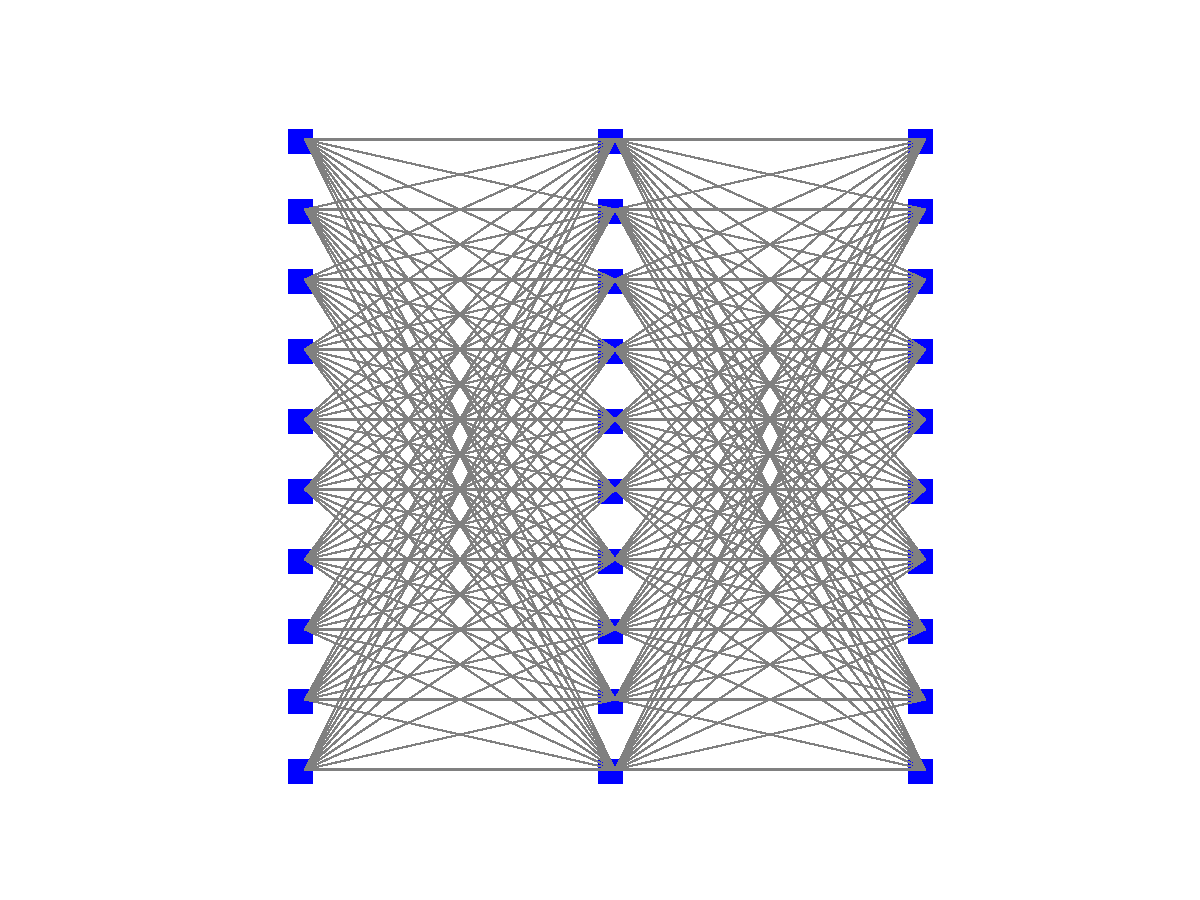
\includegraphics[width=0.8\textwidth]{images/img9}
  	\caption{مراحل طراحی معماری یک پردازنده}
  	\label{مراحل طراحی معماری یک پردازنده}
  \end{figure}
  
  معمولا در ابتدای کار، طراحی در سطح بالا به صورت رفتاری\footnote{Behavioral} با ابزار ها و شبیه‌ساز هایی مثل GEM5 یا SimpleScaler انجام می‌شود. همچنین در این مرحله خوب است که طراحی انجام شده به وسیله زبان‌ های توصیف سخت‌افزار مانند VHDL ، Verilog و SystemC شبیه‌سازی شود تا از صحت عملکرد و سنتز ‌پذیری طراحی مطمئن شویم.
  
  پس در این فاز از طراحی، شبیه‌ساز هایی که اینجانب به عنوان مدیر تیم به هم‌تیمی هایم پیشنهاد می‌دهم، شبیه‌ساز GEM5 و زبان توصیف سخت افزار SystemC است.
  
  در فاز دوم طراحی، پس از شبیه‌سازی رفتاری پردازنده، می‌بایست سلسله مراتب حافظه پردازنده را طراحی کنیم. سلسله مراتب حافظه شامل طراحی و مدلسازی حافظه اصلی پردازنده و حافظه‌های پنهان است. پس طراحی حافظه را به دو دسته تقسیم می‌کنیم:
  
  \begin{enumerate}
  	\item طراحی cache ها
  	\item طراحی حافظه اصلی
  \end{enumerate}
  
    \begin{figure}[h]
  	\centering
  	\includegraphics[width=0.8\textwidth]{images/img19}
  	\caption{ساختار پردازنده Barcelona AMD}
  	\label{ساختار پردازنده Barcelona AMD}
  \end{figure}
  
  برای طراحی Cache ها از شبیه‌ساز CACTI استفاده می‌کنیم چرا که این شبیه‌ساز صرفا مختص به مدلسازی و طراحی سلسله مراتب Cache هاست و تحلیل دقیق و جامعی از پارامتر های Cache ارائه می‌دهد.
  
  برای شبیه‌سازی و تحلیل حافظه اصلی مدار، به دلیل آنکه می‌بایست از حافظه‌های نو ظهور برای بهبود عملکرد پردازنده استفاده شود، شبیه‌ساز NVSIM را به تیمم پیشنهاد می‌دهم. چرا که این شبیه‌ساز جدید ترین و بروز ترین حافظه ها را پشتیبانی می‌کند.
  
  به دلیل آنکه صرفا هدف ما طراحی پردازنده‌ست، از بررسی شبیه‌ساز ها برای طراحی حافظه‌های RAM جانبی خودداری می‌کنیم اما اگر میخواستیم این بخش را نیز طراحی کنیم، می‌توانیم از شبیه‌ساز DRAMSIM استفاده کنیم.
  
  پس از تحلیل و طراحی سلسله مراتب حافظه با شبیه‌ساز های پیشنهاد شده «CACTI و NVSIM و DRAMSIM» می‌بایست در فاز بعدی، هر دو قسمت قبل را در سطح مدار تحلیل و تست کنیم.
  
  بهترین، دقیق ترین و کامل ترین ابزار برای شبیه‌سازی انواع مدارهای دیجیتال و آنالوگ شبیه‌ساز HSPICE است. این ابزار امکانات و تحلیل های بسیار جامعی از مدار با ما ارائه می‌کند. پس پیشنهاد بنده در این فاز، استفاده از شبیه‌ساز HSPICE است.
  
  در فاز آخر اگر سه فاز قبلی را با موفقیت پشت سر گذاشته باشیم و بخواهیم پروسسور طراحی شده را بسازیم، می‌بایست عملیات Routing پروسسور را انجام دهیم و در نهایت مدل طراحی شده را به کارخانه های Fabrication بدیم تا آن را برای ما بسازند. در این فاز شبیه‌ساز Cadence را برای تحلیل نهایی، Placement و Routing به هم‌تیمی هایم پیشنهاد می‌دهم. \\ \\ \\ \\ \\
 
 





 
 
 \question 
 یکی از ابزار‌هایی که برای شبیه‌سازی مدار‌های دیجیتال و آنالوگ و عمدتا بانک های حافظه به کار می‌رود، شبیه‌ساز HSPICE است. بر این اساس به سوالات زیر پاسخ دهید.
 
 \begin{enumerate}
 	\item دلایل ظهور شبیه‌ساز های دیگر توسعه یافته با زبان های C++ و Python و ... چیست؟ \\ \\
 	شاید این قیاس درستی نباشد که بگویم چرا شبیه‌ساز های سطح بالا توسعه داده شده است. این را از این جهت عرض می‌کنم که شبیه‌ساز HSPICE کاربرد بسیار گسترده ای در الکترونیک دارد و در این گزارش صرفا بخش بسیار کوچکی از کاربردهای آن یعنی طراحی سلول های حافظه را بررسی کردیم. به همین دلیل توسعه شبیه‌ساز های جدید بدین معنا نیست که جایگزین HSPICE بشوند. عمدتا شبیه‌ساز های جدید تمرکز بر روی افزایش سرعت تحلیل و افزایش راحتی رابط کاربری ابزار دارند.
 	
 	برای مثال شبیه‌ساز HSPICE سینتکس بسیار راحت اما بد قلقی دارد و زمان زیادی را میطلبت برای آنکه استفاده از آن برای کاربر راحت شود.
 	
 	همچنین شبیه‌ساز HSPICE ابزاری‌ست غیر رایگان و برای استفاده از آن می‌بایست لایستس آن را از شرکت Synopsys خریداری کنیم\footnote{هر چند که ما در ایران آن را کرک می‌کنیم و به رایگان استفاده می‌کنیم، ولی خب :) }
 	می‌توان گفت دلیل دیگر توسعه شبیه‌ساز های جدید م عمدتا متن باز به همین دلیل است که استفاده و توسعه شبیه‌ساز راحت باشد. چرا که با ظهور تکنولوژی های جدید و حافظه های نو ظهور، مدت زیادی طول خواهد کشید تا شرکت Synopsys تنظیمات شبیه سازش را با تکنولوژی جدید بروز کند اما اگر ابزار متن باز وجود داشته باشد، فرآیند بروزرسانی و توسعه ابزار برای تکنولوژی جدید سریعتر انجام خواهد شد. \\ \\ \\
 
 	\item درمورد اهمیت پیاده‌سازی با استفاده از ابزار‌هایی مانند HSPICE بحث کنید.\\ \\
 	ابزار های خانواده SPICE مانند PSPICE ، HSPICE ، LTSPICE و Cadence عضو جدایی ناپذیر طراحی مدارهای الکترونیکی هستند. چرا که برای تحلیل های زمانی، فرکانسی، انرژی مصرفی و ... طراحی انجام شده به این ابزار ها نیاز داریم.
 	
 این ابزار ها به دلیل آنکه شرکت های معتبر و نامداری در این زمینه از آنها پشتیبانی می‌کنند، بسیار دقیق هستند و کوچیکترین جزئیات را می‌توان با آنها شبیه‌سازی کرد.
 
 شاید مهمترین دلیل استفاده از این ابزار ها را می‌توان به صورت زیر بیان کرد:\\
 این ابزار ها مدارات را در پایین ترین سطح تجرید یعنی در سطح ترانزیستور شبیه‌سازی می‌کنند و تمام پدیده‌های غیر ایده‌آل ترانزیستور را مدل می‌کند. این امر از این جهت اهمیت دارد که وقتی شبیه سازی را در سطح بالا و بدون درنظر گرفتن ریز ترین جزئیات انجام میدهیم همه چیز ایده‌آل است اما وقتی به سطوح تجرید پایین تر می‌آییم، اثرات غیرخطی قطعات، محدودیت های ساخت و ... بر روی طراحی انجام شده اثر می‌گذارند و می‌بایست طراحی را مجددا با شرایط و امکانات موجود با این ابزار ها تحلیل و شبیه سازی کنیم.
 
 به عبارتی دیگر می‌توان گفت ابزار‌های نام برده نظیر HSPICE نزدیک ترین نتایج را نسبت به دنیای واقعی به طراحان گزارش می‌دهند.
 \end{enumerate}
 
 \end{questions}

\end{document}